\section{Data}
\label{sec:data}

\subsection{Rooftop fleet}
\label{sec:data-fleet}

The fleet comprises 33 residential PV systems in Belgium whose owners publish inverter data on PVOutput.org (Fig.~\ref{fig:fleet}). It spans 49.70--51.31$^\circ$N and 2.82--5.78$^\circ$E, about 180~km north--south and 210~km east--west, in five regions: the West Flanders coast (7 systems), Antwerp (8), Brussels and the centre (8), Li\`ege (6) and the Ardennes (4). Rated capacity ranges from 2.04 to 10.53~kW$_\mathrm{p}$ (median 4.69, total 169.7~kW$_\mathrm{p}$). Five-minute generation is averaged to 15-min means. The study window runs from 1 April 2024 to 31 May 2026 and gives 1,158,011 valid daylight records. A slot counts as daylight when modelled clear-sky GHI exceeds 5~W\,m$^{-2}$, which removes night-time zeros that would otherwise inflate every metric. One further system (12293) was excluded during data preparation. System 81376 is retained here and treated in Section~\ref{sec:res-config}.

\begin{figure}[!htb]
\centering
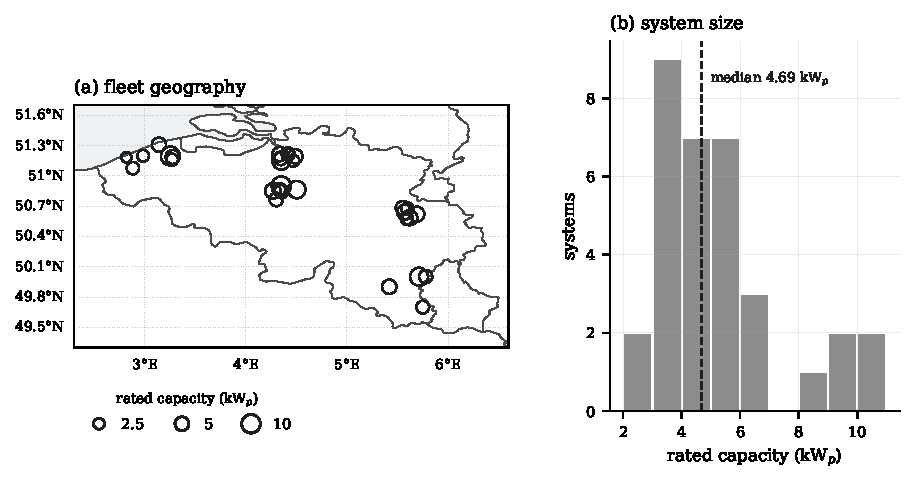
\includegraphics[width=\textwidth]{figures/fig1_fleet.pdf}
\caption{Study fleet. (a) Location of the 33 systems; marker area is proportional to rated capacity. (b) Distribution of rated capacity.}
\label{fig:fleet}
\end{figure}

\subsection{Installation metadata}
\label{sec:data-meta}

Owner-reported tilt, azimuth, rated capacity and inverter rating all enter the model (Section~\ref{sec:methods}), and none survives inspection intact (Fig.~\ref{fig:metadata}). Nine systems report a tilt of 1$^\circ$ or less, three of them exactly 0$^\circ$. Nine flat roofs in a sample of 33 Belgian houses is implausible, and the round values indicate unfilled fields. \citet{Killinger2018} filtered such entries; our pipeline used them as reported, so the transposition for these nine systems uses a near-horizontal plane. Azimuth is recorded only as a compass sector and takes three values: south (17 systems), south-west (9) and south-east (7). No east- or west-facing roof is present, and 180$^\circ$ stands for both a true southern aspect and an unreported one.

Rated capacity has the subtler problem. The ratio of each system's 99th-percentile output, $P_{99}$, to its nameplate capacity $C_\mathrm{p}$ has median 0.794 and range 0.568--1.273, a 2.24-fold spread in what full output means. Inverter clipping does not explain it, although DC capacity exceeds the inverter rating for 26 systems. On the 31 systems with a plausible inverter rating, the capacity ratio correlates with the inverse DC/AC ratio at only +0.17, and normalising by inverter rating instead of nameplate raises the coefficient of variation of $P_{99}$ from 0.157 to 0.342.
%% Clipping test reproduced from exp5_loso_per_system.csv + systems_metadata.csv; 100651 (330 W inverter entry) and 73542 (no rating) excluded.

\begin{figure}[!htb]
\centering
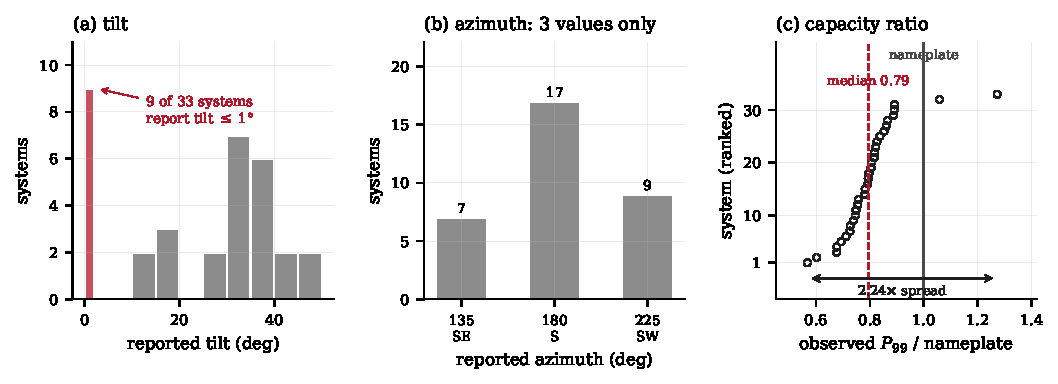
\includegraphics[width=\textwidth]{figures/fig2_metadata.pdf}
\caption{Metadata quality. (a) Reported tilt; nine systems report 1$^\circ$ or less (highlighted). (b) Reported azimuth takes three values. (c) Observed $P_{99}$ relative to nameplate capacity, ranked.}
\label{fig:metadata}
\end{figure}

\subsection{Weather forecasts}
\label{sec:data-nwp}

Day-ahead forecasts come from the Open-Meteo archive of operational NWP, retrieved with the \texttt{previous\_day1} suffix so that each value is the forecast issued one day before the target. The archive also holds analysis fields, which would be unavailable to a real forecast; none enters the features. The primary model is ECMWF IFS at 0.25$^\circ$. DWD ICON, NOAA GFS, M\'et\'eo-France, DMI and the UK Met Office supply the same variables at the same lead time, with full coverage except the Met Office (83.4\%). Seven successive ECMWF runs (\texttt{previous\_day1} to \texttt{previous\_day7}) form a lagged ensemble.

Hourly irradiance is mapped to the 15-min grid through the clear-sky index. GHI is divided by modelled clear-sky GHI with a 1~W\,m$^{-2}$ guard against division by zero, the index is interpolated linearly, and the result is multiplied by the 15-min clear-sky value. This keeps the shape of the solar curve, which direct interpolation of irradiance would flatten. The choice of clear-sky model affects downstream results \citep{Yang2020a}; we use Ineichen--Perez \citep{Ineichen2002} through pvlib \citep{Holmgren2018}.

\subsection{Reference irradiance}
\label{sec:data-ref}

Irradiance forecasts are scored against two references. ERA5 \citep{Hersbach2020} follows common practice in distributed-PV studies. SARAH-3 \citep{Pfeifroth2024,Pfeifroth2023} is the independent reference (Section~\ref{sec:rw-reference}), with 99.2\% coverage over the study window. No ground pyranometer is available for this fleet.

\subsection{Data splits}
\label{sec:data-splits}

The data are split chronologically: training from 1 April 2024 to 11 September 2025 (810,614 records), validation to 14 February 2026 (173,702) and test to 31 May 2026 (173,695). Validation is used only for hyperparameter selection and recalibration, never for reporting. Every system appears in all three partitions, so this split measures a fleet already under management and is an upper bound for a new installation. Deployment is measured separately by leave-one-system-out evaluation (Section~\ref{sec:meth-loso}).
